% ============================================================
\chapter{モメンタム}\label{ch:momentum}

モメンタムは、過去によく上がった銘柄が、その後もしばらく上がりやすいという傾向である。研究の歴史が長く、ビューの材料として使いやすい一方で、まれに大きく崩れる（急落する）。この章では、モメンタムの性質と急落を Kenneth French のデータで確かめ、急落を和らげるボラティリティの調整を再計算する。そのうえで、セクターのモメンタムを BL のビューにして試す。最後に、LLM の予想が先月の値動きの写しになっていること（『総合報告書』）を、モメンタムの観点から読み直す。

\section{モメンタムの研究}

\begin{itemize}
\item Jegadeesh と Titman（1993）は、過去 3〜12 か月によく上がった銘柄を買い、下がった銘柄を売る戦略が、その後 3〜12 か月にわたって利益を上げることを示した。直近の 1 か月は、逆に戻りやすい（短期の反転、Jegadeesh 1990）ので、過去 12 か月から直近 1 か月を除いた「12--1 か月」のリターンで順位を付けるのがふつうである。
\item Carhart（1997）は、これをファクター（UMD）にし、投資信託の成績の説明に使った。Kenneth French のデータのモメンタム・ファクターも、時価総額と過去のリターン（12〜2 か月前）で分けた 6 つのポートフォリオから作られている。
\item Asness、Moskowitz、Pedersen（2013）は、モメンタムが国や資産クラスを越えて見られ、割安さ（バリュー）のファクターと負の相関を持つことを示した。
\end{itemize}

\section{急落}

\begin{paperbox}[Daniel and Moskowitz（2016）, \textit{Momentum Crashes}, Journal of Financial Economics 122(2)]
モメンタムの大きな損失は、まれだが集中して起きる。急落は、市場が大きく下がり、ボラティリティが高い「パニックの状態」のあとで、市場が反発する時期に起きる。下がり続けた銘柄（ベータが高くなっている）が、反発の局面で大きく上がるためである。急落は、ある程度予想できる。
\end{paperbox}

\begin{table}[htbp]
\centering
\caption{モメンタム・ファクターの最悪の月（月次 \%）と、ボラティリティで調整した場合。調整の倍率は、前月末までの 126 取引日の実現ボラティリティから決めた（次の節）。}
\label{tab:mom-worst}
\tabin{mom_worst}
\end{table}

\tabref{tab:mom-worst} のとおり、最悪の月は \V{mom.worst.month} の \V{mom.worst}\% である。2009 年 4 月の \V{mom.2009}\% は、リーマン・ショックのあとの反発の局面で、Daniel と Moskowitz の言う急落の典型である。

\section{ボラティリティで規模を調整する}

\begin{paperbox}[Barroso and Santa-Clara（2015）, \textit{Momentum Has Its Moments}, Journal of Financial Economics 116(1)]
モメンタムのリスク（ボラティリティ）は時期によって大きく変わり、しかも予想しやすい。前月までの 126 取引日の日次リターンから実現ボラティリティを見積もり、目標のボラティリティ（年率 12\%）÷ 見積もり、の倍率でポジションの大きさを決める。1927〜2011 年で、シャープレシオは 0.53 から 0.97 に上がり、急落のリスクが大きく下がった。
\end{paperbox}

この方法を、Kenneth French の日次と月次のモメンタム・ファクターで再計算した。月 $t$ の倍率は、前月末までの 126 取引日の日次リターンの 2 乗の平均に 21 を掛けた月次の分散 $\hat\sigma_t^2$ から、$0.12/\sqrt{12}\,/\,\hat\sigma_t$ とした。

\begin{table}[htbp]
\centering
\caption{モメンタム・ファクターの成績と、ボラティリティで調整した場合（年率 \%、シャープレシオはリスクフリーを引かない比）。尖度は超過尖度。}
\label{tab:mom-bsc}
\tabin{mom_bsc}
\end{table}

\begin{figure}[htbp]
\centering
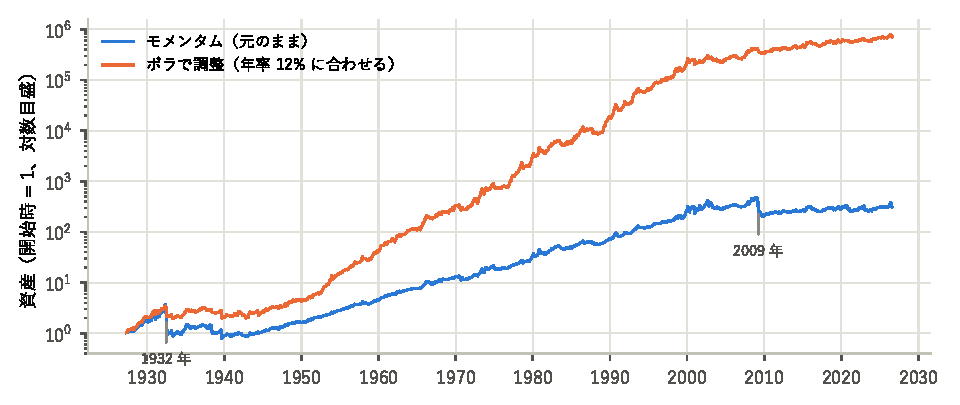
\includegraphics[width=0.95\linewidth]{fig_mom_long.pdf}
\caption{モメンタム・ファクターの累積（対数目盛）。ボラティリティで調整すると、1932 年と 2009 年の急落が小さくなり、長期の成長も大きくなる。}
\label{fig:mom-long}
\end{figure}

\tabref{tab:mom-bsc} と\figref{fig:mom-long} から分かることを挙げる。

\begin{itemize}
\item 1927〜2011 年では、シャープレシオは \V{mom.sh.sub} から \V{mom.sh.sub.sc} に上がった。Barroso と Santa-Clara の 0.53 から 0.97 とほぼ同じである（期間の始まりと、データの版がわずかに違う）。
\item 全期間（\V{mom.start}〜\V{mom.end}）でも、\V{mom.sh.all} から \V{mom.sh.all.sc} に上がった。最大の下落は \V{mom.dd}\% から \V{mom.dd.sc}\% に縮んだ。
\item 2009 年 4 月の倍率は \V{mom.2009.scale} で、損失は \V{mom.2009}\% から \V{mom.2009.sc}\% になった。急落の前に、すでにボラティリティが高くなっていたので、ポジションが小さくなっていた。
\item 2015 年以降のモメンタムは弱く、調整前のシャープレシオは 0.2 程度である。
\end{itemize}

\subsection*{BL の言葉で言うと}

ボラティリティで規模を調整することは、BL では「モメンタムのビューの確信度を、モメンタム自身の最近のボラティリティに応じて変える」ことに当たる。モメンタムの期待リターン（平均）はボラティリティほど大きく変わらないので、ボラティリティの高い時期にはシャープレシオが下がり、ビューの採用率を下げるのが理にかなう。\chapref{ch:macro} で見た「$\Omega$ だけを速く動かす」と違い、ここでは「ボラティリティの高い時期には予想（モメンタムの順位）の価値が下がる」という裏付けがある。

\section{取引戦略をビューにする研究}

\begin{itemize}
\item Fabozzi、Focardi、Kolm（2006）は、モメンタムのような取引戦略を BL のビューとして組み込む枠組みを示した（\textit{Incorporating Trading Strategies in the Black--Litterman Framework}, Journal of Trading 1(2)）。この資料では本文を確認できなかった。
\item Bessler、Opfer、Wolff（2017）は、過去のデータから作るビュー（標本に基づく BL）を、世界の株式・債券・商品の指数（1993〜2011 年）に当てはめた。BL のポートフォリオは、1/N、平均分散、Bayes--Stein、最小分散のどれよりも、標本外のシャープレシオが高かった。リスク回避度、投資の制約、取引費用を変えても同じだった。理由として、期待リターンの見込みが安定し、推定の誤差が小さく、回転率が低いことを挙げている。
\end{itemize}

\section{セクターのモメンタムを BL で試す}

本プロジェクトのセクター ETF（最大 11 セクター）で、モメンタムのビューを BL に入れて検証した。

\begin{itemize}
\item \textbf{期間}：判断日は 2016 年 1 月〜2026 年 8 月の各月末（\V{sm.months} か月）。翌月のリターンで評価する。
\item \textbf{ベンチマーク}：その日の \SP{} の構成銘柄の時価総額をセクターごとに合計した比率（ETF のあるセクターだけ）。
\item \textbf{均衡}：$\Sigma$ は過去 252 日の日次リターンの縮小推定を 21 倍した月次の共分散。$\delta=2.5$。
\item \textbf{点数}：12--1 か月のモメンタムを、セクターの間で標準化した $z$。
\item \textbf{IC}：その月までに分かっている、点数と翌月のリターン（セクターの平均を引く）の相関の平均。最初は 0.05 を 24 か月分の重みで混ぜ、負なら 0 とする。
\end{itemize}

比べた戦略は 3 つである。

\begin{enumerate}
\item \textbf{IC で縮めたビュー}：$\mu=\Pi+\IC_t\cdot\sigma\cdot z$（Grinold の式。市場版の BL で $\omega=\sigma^2(1/\IC^2-1)$ と同じ）。
\item \textbf{IC ＋ ボラティリティで調整}：上の $\IC_t$ に、モメンタム・ファクターのボラティリティの倍率（前の節、上限 1.5）を掛ける。
\item \textbf{過去の平均がそのまま続く}：$\mu=\Pi+(\text{12--1 か月のリターン})/11$。過去 11 か月の月平均のリターンが、そのまま来月も続くとみる（採用率 100\%）。
\end{enumerate}

どれも、空売りなし・全額投資で $\mu\T w-\frac{\delta}{2}w\T\Sigma w$ を最大にした。

\begin{figure}[htbp]
\centering
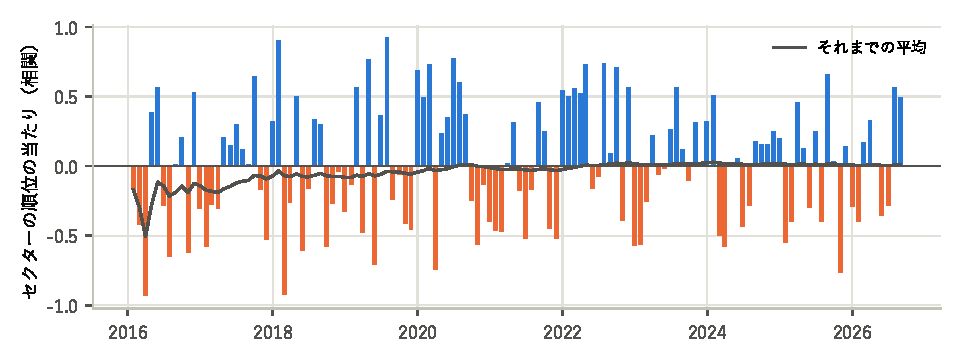
\includegraphics[width=0.95\linewidth]{fig_secmom_ic.pdf}
\caption{セクターのモメンタムの当たり具合（月ごとの、点数と翌月のリターンの相関）と、それまでの平均。}
\label{fig:secmom-ic}
\end{figure}

\begin{table}[htbp]
\centering
\caption{セクターのモメンタムの BL（\V{sm.start}〜\V{sm.end}、年率 \%）。TE と IR はベンチマークに対するもの、$t$ 値は月次の超過リターンの平均の $t$ 値、回転率は月平均、実質数は $1/\sum w^2$ の平均。}
\label{tab:secmom}
\tabin{secmom}
\end{table}

\begin{figure}[htbp]
\centering
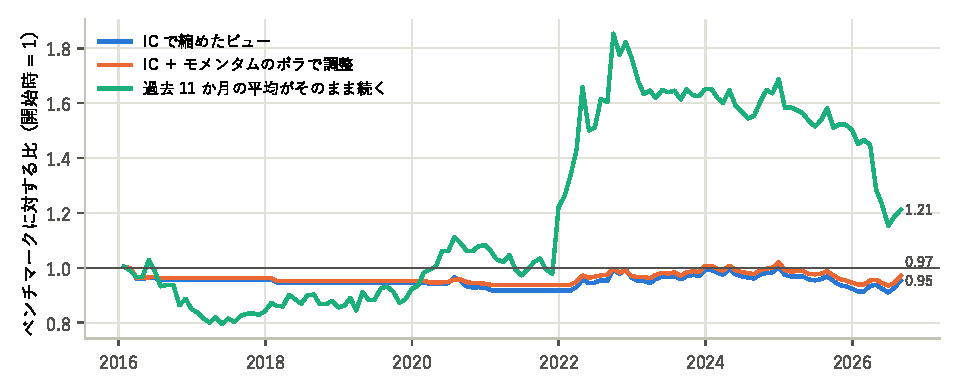
\includegraphics[width=0.95\linewidth]{fig_secmom_cum.pdf}
\caption{ベンチマークに対する累積の比。}
\label{fig:secmom-cum}
\end{figure}

結果は次のとおりである。

\begin{itemize}
\item セクターのモメンタムの当たり具合は、平均 \V{sm.cic.mean}（$t$ 値 \V{sm.cic.t}、128 か月のうち \V{sm.cic.pos} か月がプラス）で、ほとんど 0 だった（\figref{fig:secmom-ic}）。セクターは 10 前後しかないので、月ごとの相関は $\pm1$ の近くまで大きくぶれる。
\item IC で縮めたビューは、採用率がほとんど 0 になるので、ベンチマークに近い比率になった。TE は \V{sm.icv.te}\%、IR は \V{sm.icv.ir}（$t$ 値 \V{sm.icv.t}）。ボラティリティで調整した版も同じような結果である。
\item 過去の平均がそのまま続くとみる戦略は、実質 1 セクター程度に集中し、TE は \V{sm.naive.te}\% と大きい。2022 年に大きく勝ち（この年はエネルギーのセクターが大きく上がった）、その後に負けを重ねた（\figref{fig:secmom-cum}）。IR は \V{sm.naive.ir}（$t$ 値 \V{sm.naive.t}）で、偶然と区別できない。
\end{itemize}

当たり具合が 0 に近いビューを正しく縮めると、BL はほとんど何もしない。これは失敗ではなく、BL が設計どおりに働いた結果である。逆に、縮めずに入れた戦略の大きな勝ち負けは、ビューの価値ではなく、集中の結果である。

\section{LLM の予想と短期の反転}

『総合報告書』で見たとおり、本プロジェクトの LLM の予想は、渡した月の平均リターンとの相関が平均 \V{llm.cin.mean} で、先月の値動きをほぼ写している。これは「直近 1 か月の値動きがそのまま続く」という、1 か月のモメンタムの予想である。

モメンタムの研究は、12--1 か月のモメンタムを使い、直近の 1 か月をわざわざ除く。個別の銘柄では、直近 1 か月によく上がった銘柄は翌月に戻りやすい（短期の反転、Jegadeesh 1990、Lehmann 1990）からである。LLM の予想は、この反転とは逆の向きに賭けていることになる。

ただし、本プロジェクトの DB で 2015〜2026 年の \SP{} の構成銘柄を調べると、直近 1 か月のリターンと翌月のリターンの順位相関は \V{tic.return_1m.mean}（$t$ 値 \V{tic.return_1m.t}）で、反転も継続もほとんど見られなかった（\chapref{ch:esg} の\tabref{tab:stock-ic}）。12--1 か月のモメンタムも \V{tic.momentum_12m.mean} で、効いていない。LLM の予想の当たり具合は弱い正（順位相関 \V{llm.ic.mean}）で、少なくとも 2024〜2026 年には反転に負けてはいなかった。それでも、「先月の写し」のビューに大きな確信を置く根拠は、モメンタムの研究からも、この期間のデータからも出てこない。

\begin{tipbox}[コツ：モメンタムのビュー]
\begin{enumerate}
\item 順位は 12--1 か月のリターンで付ける。直近の 1 か月は、個別の銘柄では反転しやすい。
\item ビューの大きさは IC で決める。モメンタムの IC は時期によって大きく変わり、最近 10 年は弱い。
\item モメンタム自身の最近のボラティリティが高いときは、確信度を下げる（Barroso and Santa-Clara の倍率）。急落は、下げ相場のあとの反発で起きやすい。
\item 勝ち組と負け組の差（相対ビュー）で入れ、市場全体の方向の賭けを混ぜない。
\item 縮めずに入れると、比率は少数の資産に集中し、成績は集中の結果になる。
\end{enumerate}
\end{tipbox}

\begin{keybox}[この章のまとめ]
\begin{itemize}
\item モメンタムは、まれに大きく急落する（最悪の月は \V{mom.worst}\%）。急落は、下げ相場のあとの反発の局面で起きる。
\item 実現ボラティリティで規模を調整すると、シャープレシオは \V{mom.sh.all} から \V{mom.sh.all.sc} に上がり、最大の下落は \V{mom.dd}\% から \V{mom.dd.sc}\% に縮んだ。BL では、確信度をモメンタムのボラティリティで動かすことに当たる。
\item セクターのモメンタムは 2016〜2026 年にはほとんど当たらず、正しく縮めた BL はベンチマークの近くにとどまった。
\item LLM の「先月の写し」の予想は、1 か月のモメンタムの賭けで、個別株の短期の反転とは逆の向きである。
\end{itemize}
\end{keybox}
